	\documentclass[14pt]{extreport}
\usepackage{extsizes}
	\usepackage[frenchb]{babel}
	\usepackage[utf8]{inputenc}  
	\usepackage[T1]{fontenc}
	\usepackage{amssymb}
	\usepackage[mathscr]{euscript}
	\usepackage{stmaryrd}
	\usepackage{amsmath}
	\usepackage{tikz}
	\usepackage[all,cmtip]{xy}
	\usepackage{amsthm}
	\usepackage{varioref}
	\usepackage[ margin=0.6in]{geometry}
	\geometry{a4paper}
	\usepackage{lmodern}
	\usepackage{hyperref}
	\usepackage{array}
	\usepackage{float}
	\usepackage{easytable}
	 \usepackage{fancyhdr}\usepackage{longtable}
	 \usetikzlibrary{shapes.misc}
	 \newcommand\ang[1]{$#1{}^o$}
\newlength{\taillecellule}
\setlength{\taillecellule}{2cm}
\newcolumntype{C}{@{}>{\centering\arraybackslash}p{\taillecellule}@{}}
 

	\pagestyle{fancy}
	\theoremstyle{plain}
	\fancyfoot[C]{\empty} 
	\fancyhead[L]{Interrogation chapitre 8}
	\fancyhead[R]{3 juin 2024}
	
	
	\title{Interrogation chapitre 7}
	\date{}
	
	
	\begin{document}
 \subsection*{Exercice 1}
Calculez, en détaillant les étapes sur votre copie : 

\begin{enumerate}
\item $2 - (-3) + 5 \times  2$
\item $ -2 + 3 \times 4$
\item $((5 - 4) \times 2 + 3 )\times 7 - 4$
\item $-2 - (3 - 1)$.
\end{enumerate}

\subsection*{Exercice 2}
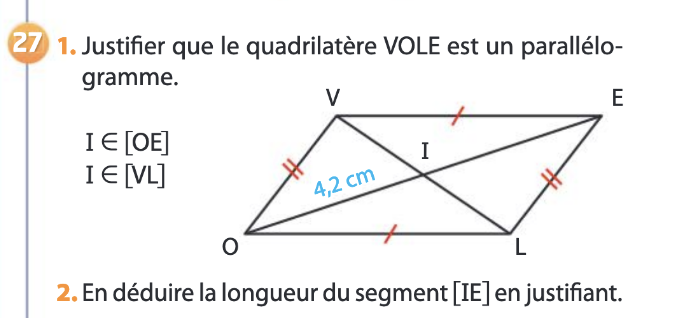
\includegraphics[scale=1]{Exo}

\subsection*{Exercice 3} % 7,5 pts

\begin{enumerate}
\item  \begin{enumerate}
	\item Tracer un triangle $ABC$ avec $AB = 8$ cm et $AC = 10$ cm (la longueur $BC$ est libre). 
	\item Placer le milieu $M$ du segment $[AB]$
	\item Tracer la droite parallèle à $(BC)$ passant par $M$. Elle rencontre $[AC]$ en un point $N$. 
	\item Tracer la droite parallèle à $(AB)$ passant par le point $N$. Cette droite coupe le segment $[BC]$ en $O$. 
\end{enumerate}
\item  Quelle est la nature du quadrilatère $MNOB$ ? Justifiez. Déduisez-en une relation entre les longueurs $MB$, $MA$ et $NO$. 
\item Démontrez alors que $MANO$ est un parallélogramme. Que peut-on en déduire des droites $(MO)$ et $(AC)$ ? Que dire des longueurs $AN$ et $MO$ ? 
\item Démontrez enfin que $MNCO$ est un parallélogramme.
\item En déduire que $MO=NC$, puis que $N$ est le milieu de $[AC]$.

\end{enumerate}
\end{document}

